
\section{Resultados}

Esta seção apresenta os resultados com dois representantes de cada classe por
figura.

\begin{figure}[htb]
  \caption{Classe homogênea: regras 136 e 36, respectivamente}
  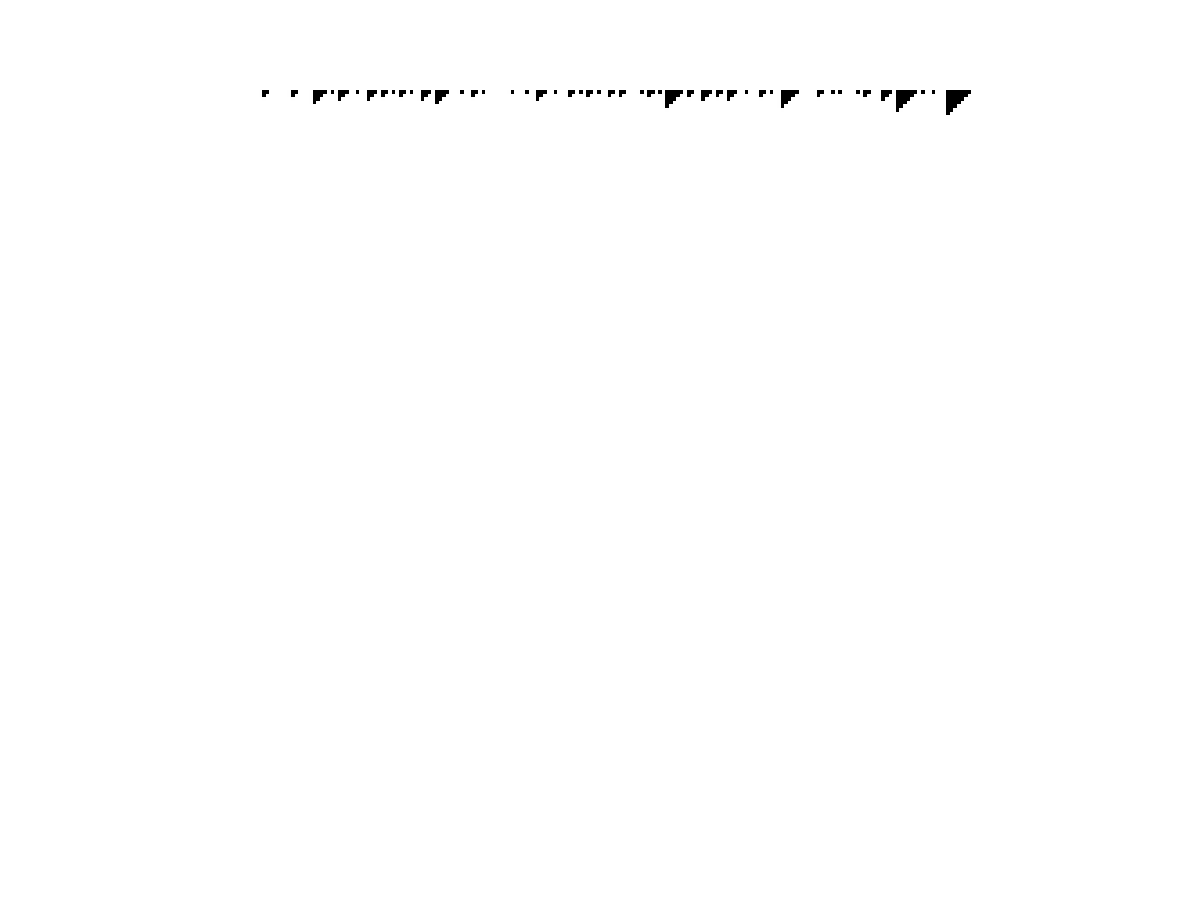
\includegraphics[width=0.5\textwidth]{figures/136.pdf}
  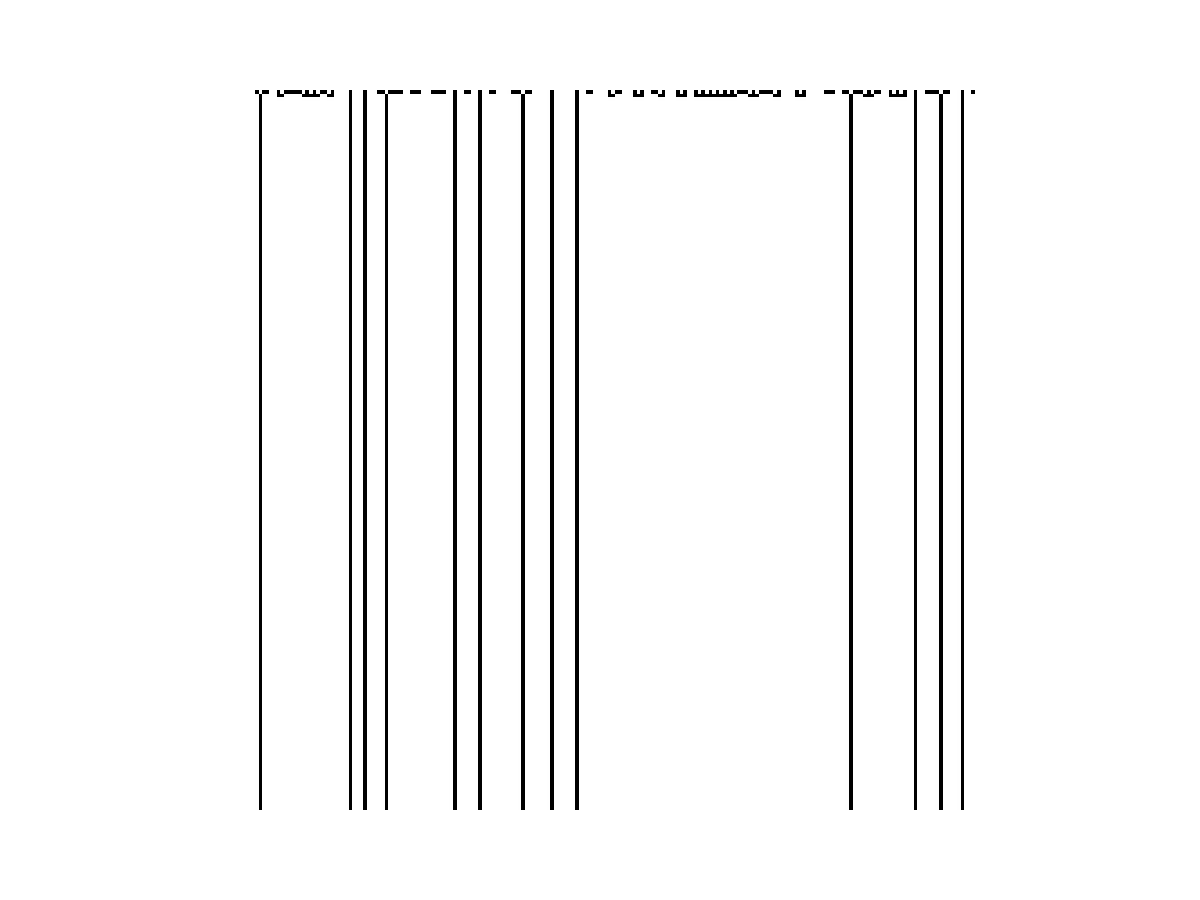
\includegraphics[width=0.5\textwidth]{figures/36.pdf}
  \label{fig:wolfram_homogeneous}
\end{figure}

\begin{figure}[htb]
  \caption{Classe periódica: regras 73 e 23, respectivamente}
  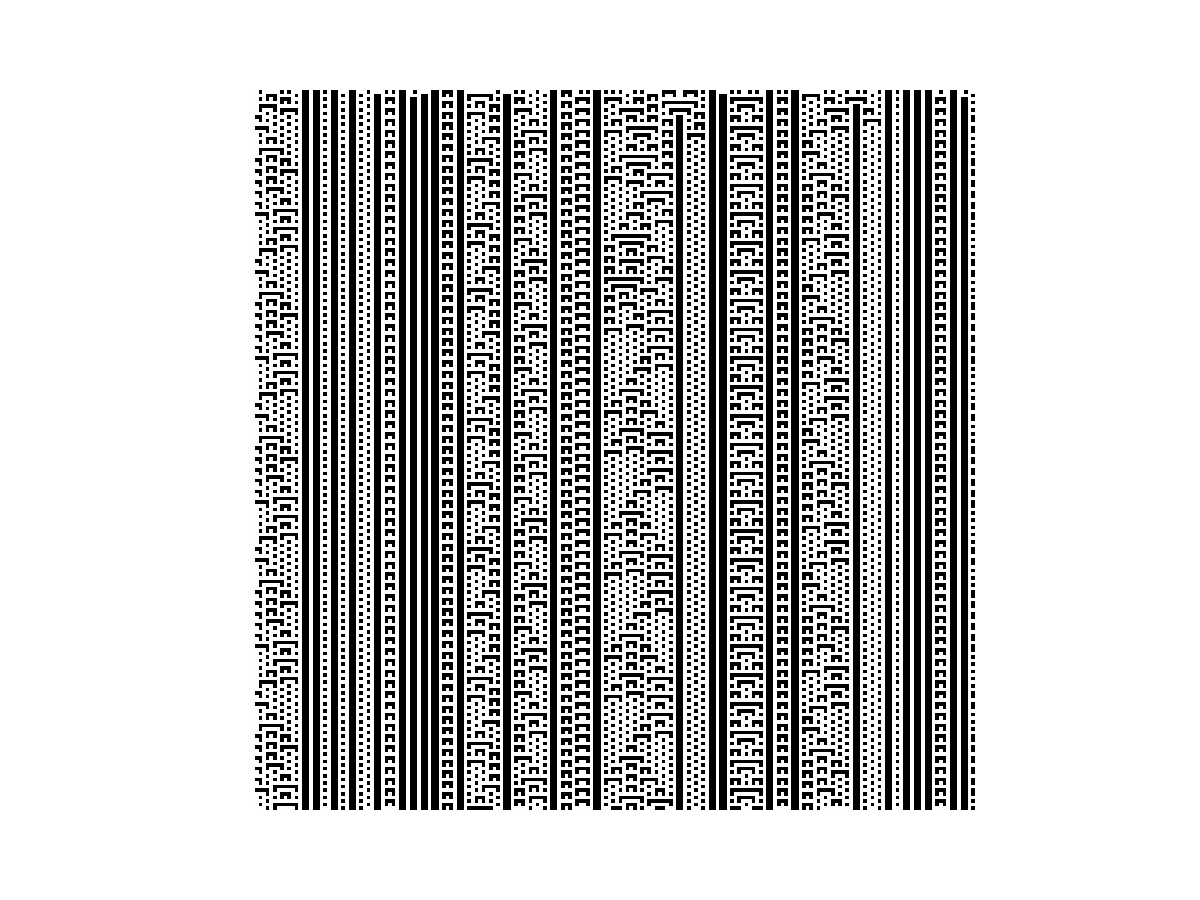
\includegraphics[width=0.5\textwidth]{figures/73.pdf}
  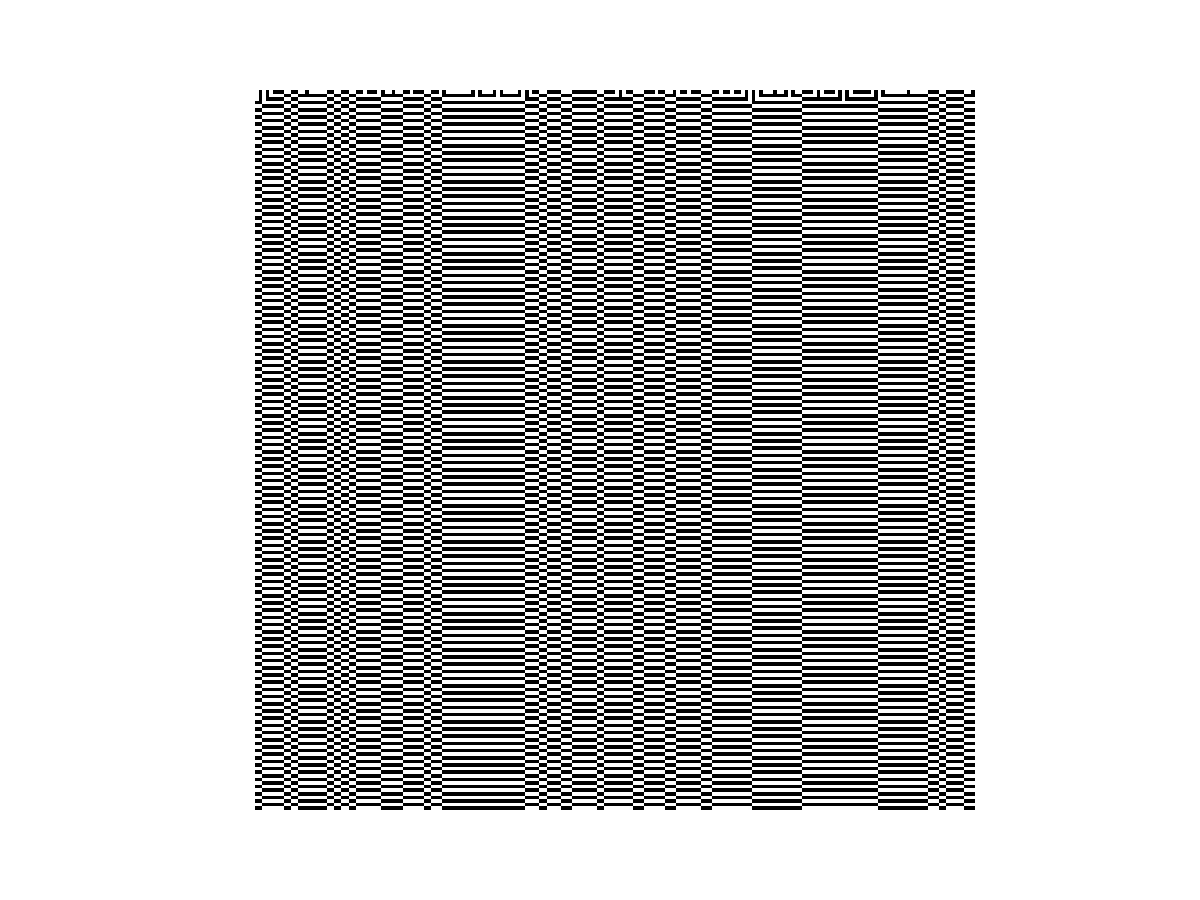
\includegraphics[width=0.5\textwidth]{figures/23.pdf}
  \label{fig:wolfram_periodic}
\end{figure}

\begin{figure}[htb]
  \caption{Classe caótica: regras 90 e 22, respectivamente}
  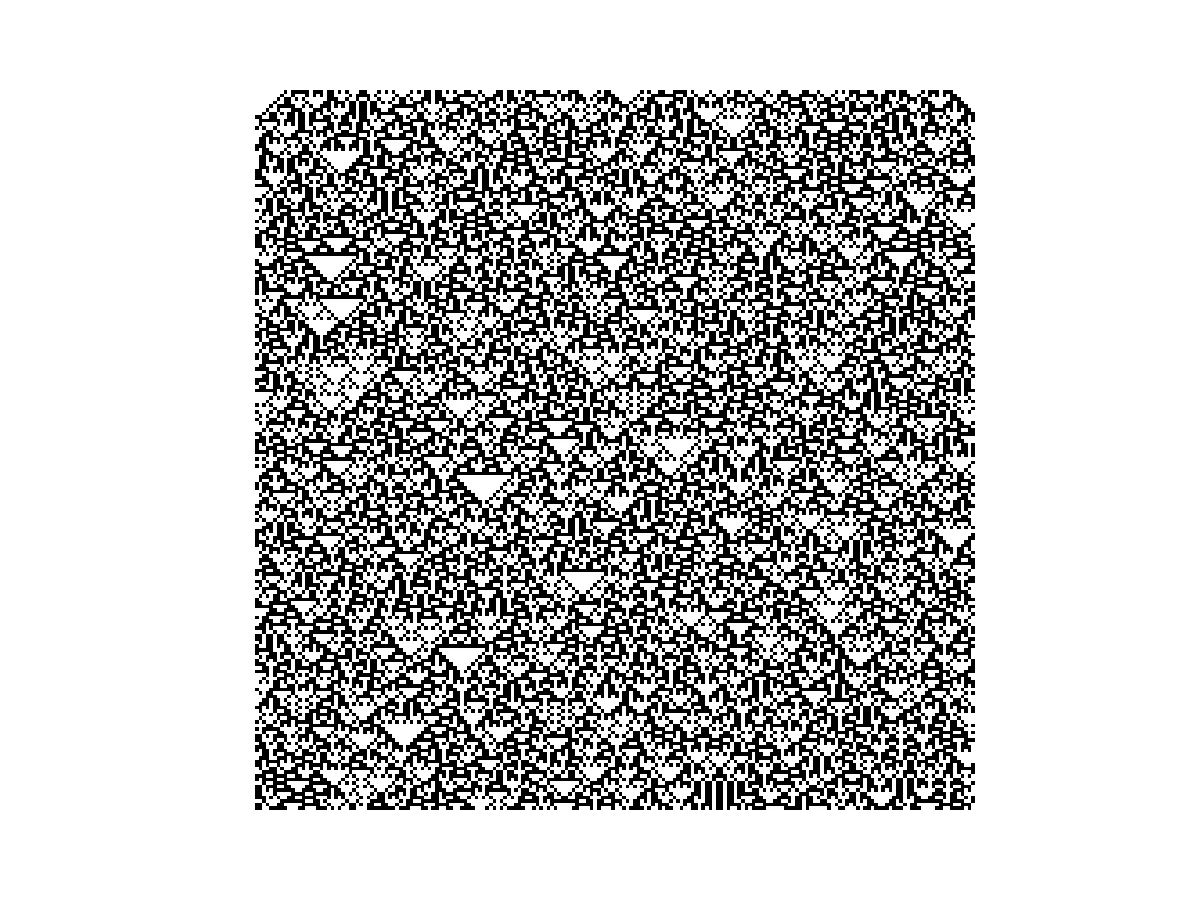
\includegraphics[width=0.5\textwidth]{figures/90.pdf}
  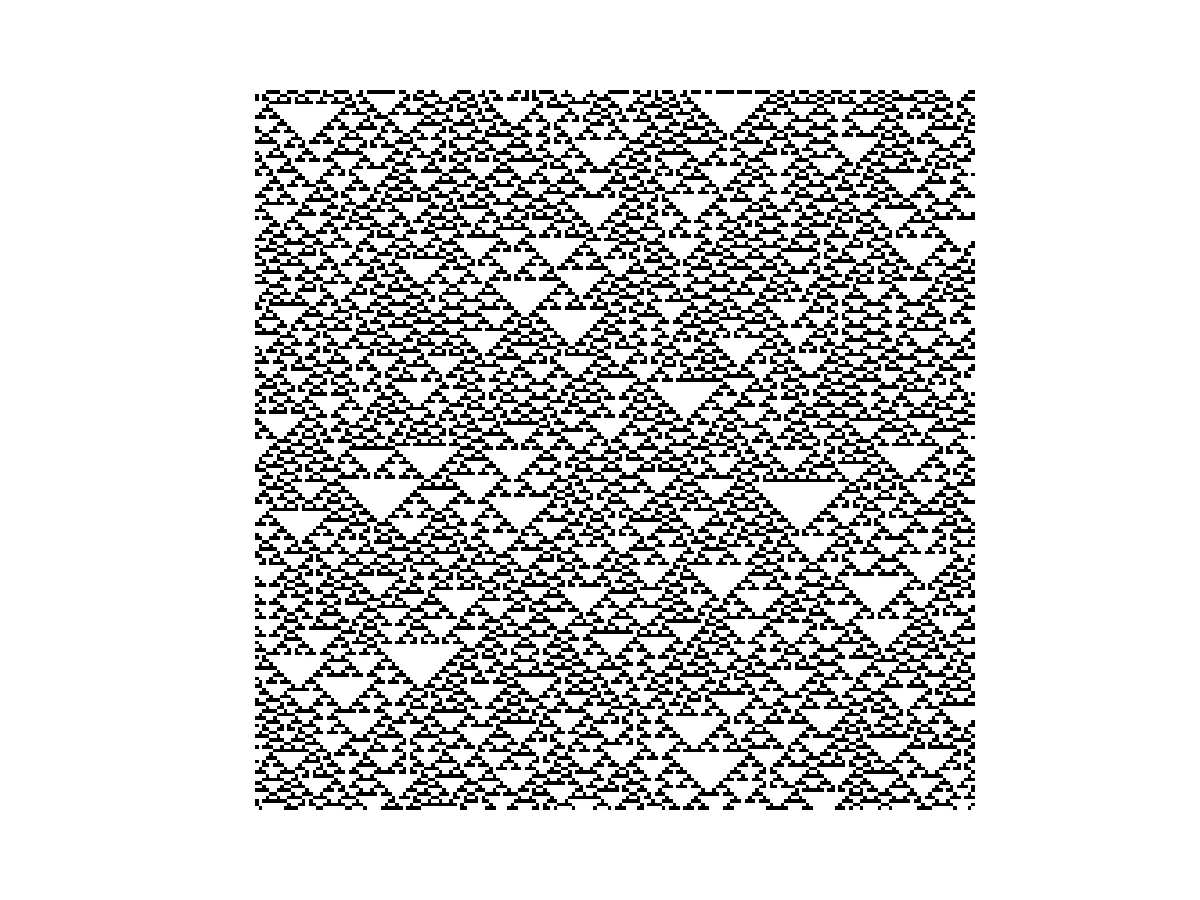
\includegraphics[width=0.5\textwidth]{figures/22.pdf}
  \label{fig:wolfram_chaotic}
\end{figure}

\begin{figure}[htb]
  \caption{Classe de estruturas complexas: regras 110 e 184, respectivamente}
  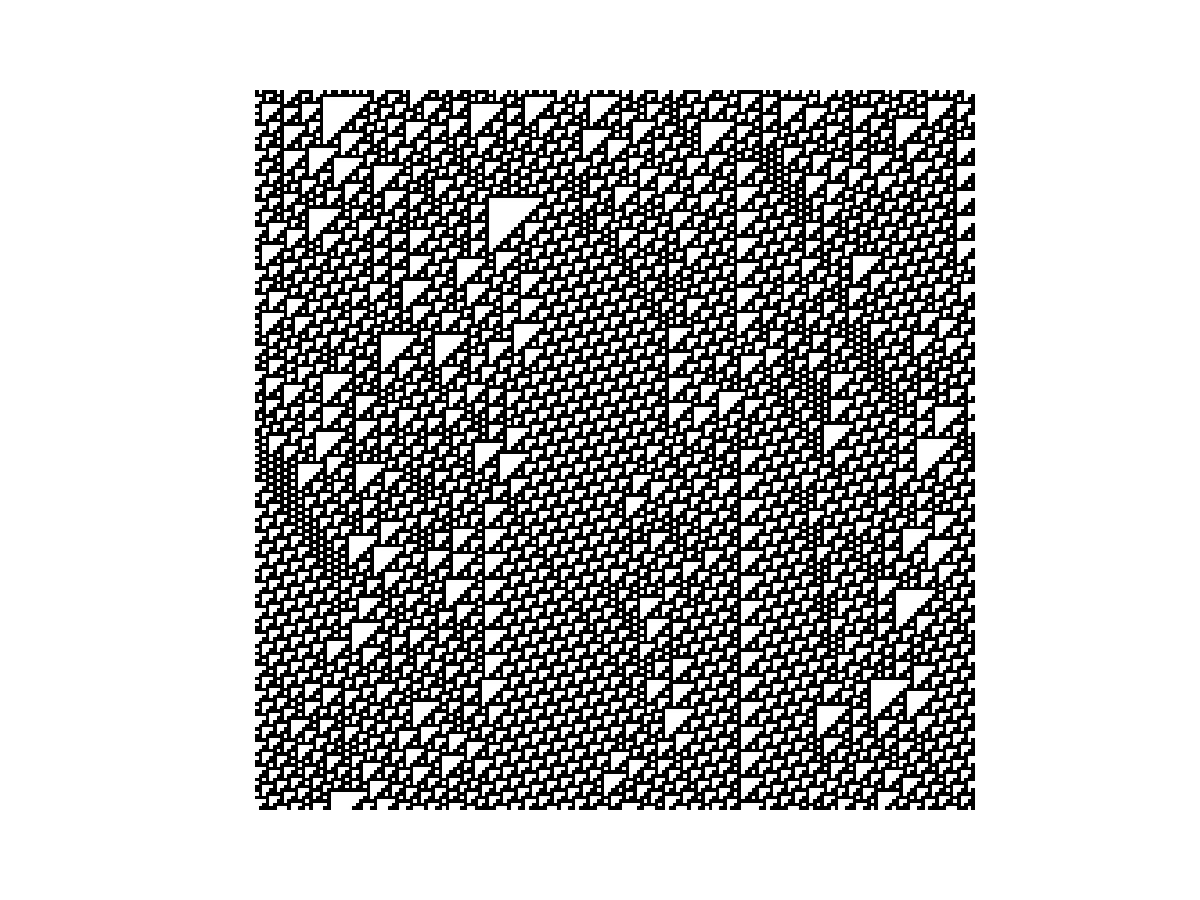
\includegraphics[width=0.5\textwidth]{figures/110.pdf}
  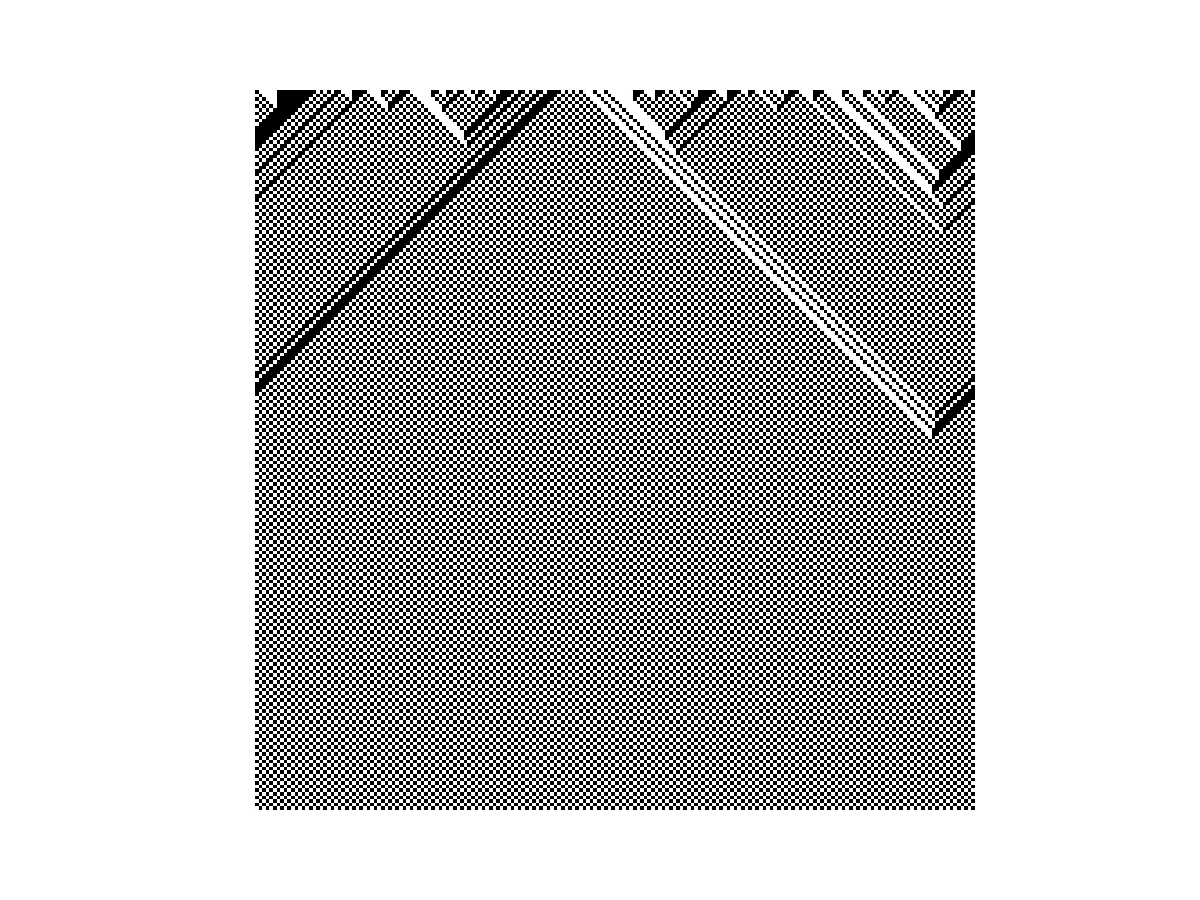
\includegraphics[width=0.5\textwidth]{figures/184.pdf}
  \label{fig:wolfram_complex}
\end{figure}
